%%%%%%%%%%%%%%%%%%%%%%%%%%%%%%%%%%%%%%%%%%%%%%%%%%%%%
%		CAP 4
%%%%%%%%%%%%%%%%%%%%%%%%%%%%%%%%%%%%%%%%%%%%%%%%%%%%%

\section[BMG con nanopart\'iculas]{BMG con nanopart\'iculas embebidas}
%\subsection{BMG con nanopart\'iculas embebidas}

\begin{frame}
  \frametitle{Introducción}
  \begin{itemize}
   \item La plasticidad es dominada por STZs que crecen y colapsan en SBs las cuales conducen a una falla frágil del material.
   \item Para homogeneizar el régimen plástico y evitar esto, la composición se modifica de diferentes maneras
  \end{itemize}
  \vspace{-1cm}
  \begin{figure}[htp]
    \centering
    \begin{tabular}{c}
      \subfloat[Nano partículas \cite{Albe13}]{
	      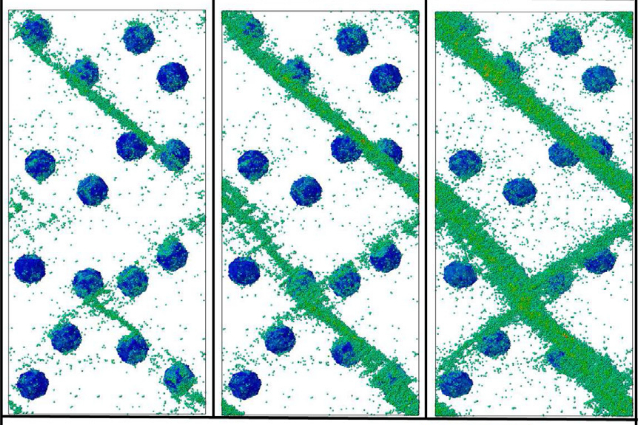
\includegraphics[width=5cm]{../Figures/Presentacion/nanoparticles_example.png}
	      \label{P:fg:B2Crystal}}
    \quad
      \subfloat[Nano vidrios \cite{Adibi13}]{
	      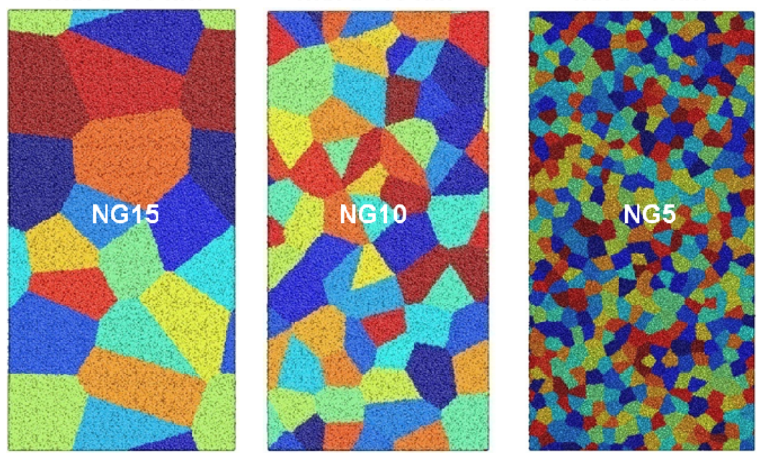
\includegraphics[width=5cm]{../Figures/Presentacion/nanoglass_example.png}
	      \label{P:fg:B2CrystalTest}}
    \end{tabular}
    \caption{BMGs con composición modificada}
    \label{P:fg:B2CuZr_Formation}
  \end{figure} 
\end{frame}

\begin{frame}
Se estudia:
 \begin{itemize}
  \item Estabilidad térmica de las nanopartículas (difusión del material cristalino en la matriz amorfa).
  \item Impacto en el comportamiento mecánico de la muestra (cambios en curvas tensión-deformación)
  \item Distribución de la tensión de corte en la muestra.
 \end{itemize}
\end{frame}
